\chapter{Die Natürliche Sprache}
Die Verarbeitung natürlicher Sprache (NLP) ist ein Teilbereich des maschinellen Lernens (ML), der sich mit natürlicher Sprache befasst, häufig in Form von Text, der selbst aus kleineren Einheiten wie Wörtern und Zeichen besteht. Der Umgang mit Textdaten ist problematisch, da unsere Computer, Skripte und Modelle für maschinelles Lernen, keinen Text im menschlichen Sinne lesen und verstehen können.
Wenn ich das Wort \enquote{Katze} lese, werden viele verschiedene Assoziationen aufgerufen - es ist ein kleines Pelztier, Fische frisst und 4 Beine hat. Aber diese sprachlichen Assoziationen sind das Ergebnis recht komplexer neurologischer Berechnungen, die über Millionen Jahre verfeinert wurden. Während unsere ML-Modelle ohne vorgefertigtes Verständnis der Wortbedeutung von vorne beginnen müssen.

\section{Textverarbeitung und Textnormalisierung}


\section{One-Hot-Codierung}
Die numerischen Werte sollten so viel wie möglich von der sprachlichen Bedeutung eines Wortes erfassen. Eine gut ausgewählte, informative Eingabedarstellung kann einen massiven Einfluss auf die Gesamtleistung des Modells haben. Worteinbettungen sind der vorherrschende Ansatz für dieses Problem und so weit verbreitet, dass ihre Verwendung praktisch in jedem NLP-Projekt angenommen wird. Unabhängig davon, ob Sie ein Projekt in den Bereichen Textklassifizierung, Sentimentanalyse oder maschinelle Übersetzung starten.

Angenommen es wird ein Modell entwickelt mit einem Wortschatz von 10.000 Wörtern. Eine Möglichkeit wäre es, ein Index aufzustellen und jedem Wort ein Integer zu geben. Dieser Integer würde dann in ein Vektor umgewandelt, wobei das este Wort einen Vektor [1, 0, 0, 0, …, 0] hätte und das also ein Vektor mit einer 1 am Anfang und  9.998 Nullen. Diese Repräsentation des Wortschatzes wird  wird als \enquote{one-hot vector encoding} bezeichnet.

Angenommen, unser NLP-Projekt erstellt ein Übersetzungsmodell und wir möchten den englischen Eingabesatz \enquote{Die Katze ist schwarz} in eine andere Sprache übersetzen. Wir müssen zuerst jedes Wort mit einer One-Hot-Codierung darstellen. Wir würden zuerst den Index des ersten Wortes \enquote{the} nachschlagen und feststellen, dass sein Index in der Vokabelliste 8676 ist. Wir könnten dann das Wort \enquote{the} unter Verwendung eines Vektors mit einer Länge von 10.000 darstellen, wobei jeder Eintrag eine 0 ist, abgesehen von dem Eintrag an Position 8676, der eine 1 ist. Wir führen diese Indexsuche für jedes Wort im Eingabesatz durch und erstellen einen Vektor, der jedes Eingabewort darstellt. Dieser Prozess generiert für jedes Eingabewort einen sehr \enquote{spärlichen} (meist null) Merkmalsvektor.

Idealerweise möchten wir, dass ähnliche Wörter wie \enquote{Katze} und \enquote{Tiger} ähnliche Merkmale aufweisen. Aber mit One-Hot-Codierung sind Vektoren für \enquote{Katze}  und \enquote{Tiger} so ähnlich wie buchstäblich jedes andere Wort. Ein weiterer Punkt ist, dass wir möglicherweise analoge Vektoroperationen für die Worteinbettungen durchführen möchten (wie z.B. \enquote{Katze} + \enquote{groß} = \enquote{Tiger}).

\begin{figure}[H]
    \centering
    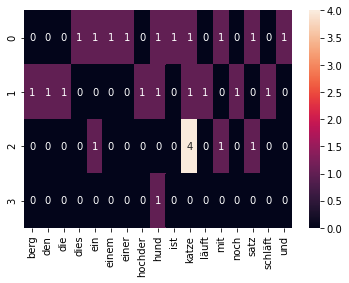
\includegraphics[width=8cm]{kapitel3/onhot.png}
    \caption[One-Hot-Codierung als Eingabematrix]{Die Grafik zeigt wie ein Beispielkorpus welches aus 5 Sätzen besteht, in einer Matrix dargestellt werden kann. Je nach Häufigkeit wird jedes Wort im Wortschaft entsprechend den Sätzen im Korpus abgebildet. Der Korpus besteht aus 5 Sätzen (\enquote{Dies ist ein Satz mit einer Katze und einem Hund.}, \enquote{Die Katze läuft den Berg hoch.}, \enquote{Der Hund schläft noch.}, \enquote{Ein Satz mit Katze Katze Katze Katze.} und \enquote{Ein Hund.}) (eigene Darstellung).}
    \label{OneHotGrafik}
\end{figure}

Wenn bei One-Hot-Codierung der Wortschatz um $n$ erhöht wird, erhöhen sich auch die Merkmalsgrößenvektoren um die Länge $n$. Die One-Hot-Vektordimensionalität entspricht der Anzahl der Wörter. Mehr Features bedeuten nämlich, dass mehr Parameter geschätzt werden müssen, und exponentiell mehr Daten benötigt werden, um diese Parameter gut genug zu schätzen, um ein einigermaßen verallgemeinerbares Modell zu erstellen (\enquote{curse of dimensionality}).

\section{Worteinbettungen}
Wenn davon ausgegangen wird, dass Wörter wie \enquote{Katze} und \enquote{Tiger} tatsächlich ähnlich sind, möchten wir diese Informationen auf irgendeine Weise an das Modell weitergeben. Dies wird besonders wichtig, wenn eines der Wörter selten ist (z. B. \enquote{Liger}), da es auf den Berechnungspfad zurückgreifen kann, den ein ähnliches, häufigeres Wort durch das Modell führt. Dies liegt daran, dass das Modell während des Trainings lernt, die eingegebene \enquote{Katze} auf eine bestimmte Weise zu behandeln, indem es sie durch Schichten von Transformationen sendet, die durch Gewichte und Bias-Parameter definiert sind. Wenn das Netzwerk schließlich \enquote{Liger} sieht und seine Einbettung \enquote{Katze} ähnelt, wird es einen ähnlichen Weg wie \enquote{Katze} einschlagen, anstatt dass das Netzwerk lernen muss, wie es vollständig von Grund auf neu zu handhaben ist. Es ist sehr schwierig, Vorhersagen über Dinge zu treffen, die das Modell noch nie zuvor gesehen hat, jedoch viel einfacher, wenn es sich auf etwas bezieht, dass es gesehen hat.

Vektoren zur Darstellung von Wörtern werden im Allgemeinen als Einbettungen bezeichnet, da das Wort in einen bestimmten Vektorraum eingebettet wird \cite*[99]{Jurafskya}.



\begin{figure}[H]
    \centering
    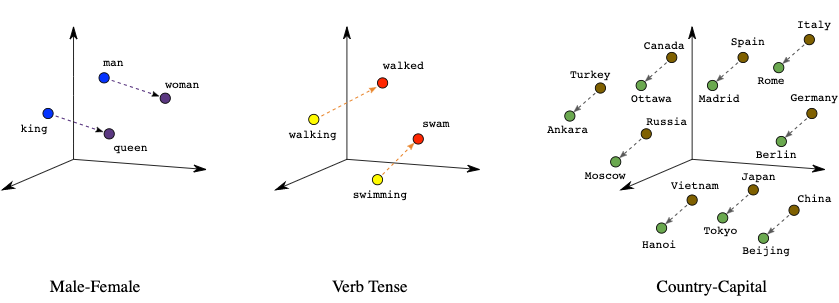
\includegraphics[width=14cm]{kapitel3/wordem.png}
    \caption[Worteinbettungen erzeugen Analogien zwischen Wörtern]{Durch Worteinbettungen können interessante Analogien zwischen einzelnen Wörtern gefunden werden. (Entnommen aus \cite*{wordemdgood})}
    \label{Word2Vex}
\end{figure}


Word2Vec \cite*{Mikolov2013} Worteinbettungen sind Vektordarstellungen von Wörtern, die normalerweise von einem Modell gelernt werden, wenn große Textmengen als Eingabe eingegeben werden (z. B. Wikipedia, Wissenschaft, Nachrichten, Artikel usw.). Diese Darstellung von Wörtern erfasst die semantische Ähnlichkeit zwischen Wörtern unter anderen Eigenschaften. Word2Vec-Worteinbettungen werden so gelernt, dass der Abstand zwischen Vektoren für Wörter mit enger Bedeutung (z. B. \enquote{König} und \enquote{Königin}) näher ist als der Abstand für Wörter mit völlig unterschiedlichen Bedeutungen (z. B. \enquote{König} und \enquote{Katze}).

Bei der One-Hot-Codierung haben die Wörter \enquote{gut} und \enquote{großartig}
Wir haben gesehen, dass bei der One-Hot-Codierung gibt es keine Projektion entlang der anderen Dimensionen. Dies bedeutet, dass \enquote{gut} und \enquote{großartig} so unterschiedlich sind wie \enquote{Tag} und \enquote{haben}, was nicht stimmt. Hier kommt die Idee, verteilte Darstellungen zu erzeugen. Intuitiv wird eine gewisse Abhängigkeit eines Wortes von den anderen Wörtern eingeführt. Die Wörter im Kontext dieses Wortes würden einen größeren Anteil dieser Abhängigkeit erhalten. In der One-Hot-Coding-Darstellung sind alle Wörter unabhängig voneinander, wie bereits erwähnt.




% DDas CBOW-Modell sagt das Mittelwort aus umgebendem Kontext vorher. Der Ansatz besteht darin, [\enquote{Die}, \enquote{Katze}, \enquote{über}, \enquote{die}, \enquote{Pfütze}] als Kontext zu behandeln und aus diesen Wörten in der Lage zu sein, das Mittelwort \enquote{gesprungen} vorherzusagen oder zu generieren. Dieser Ansatz ist die kontinuierliche Behandlung der Wörter und wird \enquote{Continuous Bag of Words} genannt. 
% Die Continuous Bag of Words (CBOW) ist eine von zwei eingeführten Modellarchitekturen des Word2Vec
% von \cite*{Mikolov2013}. Das CBOW-Modell lernt Wortrepräsentationen durch ein probabilistisches neuronales Feedforward-Netzwerk, um das Zielwort anhand der Kontextwörter vorherzusagen. Die CBOW-Architektur sagt das aktuelle Wort basierend auf dem Kontext voraus.

% Das Skip-Gram-Modell ähnelt CBOW, versucht jedoch, anstatt das Zielwort basierend auf dem Kontext vorherzusagen, die Kontextwörter innerhalb eines Radius vorherzusagen, der dem Zielwort gegeben ist. Die Skip-Gram-Architektur kehrt also die Verwendung von Ziel- und Mittelwörtern um.




\subsection{Word2Vec mit der Skip-Gram Architektur}

Wörter können als spärliche, lange Vektoren mit vielen Dimensionen dargestellt werden. Eine alternative Methode ist die Darstellung eines Wortes mit der Verwendung von kurzen Vektoren, mit einer Länge von vielleicht 50-1000 und einer großen dichte (die meisten Werte sind nicht Null). Es stellt sich heraus, dass dichte Vektoren in jeder NLP-Aufgabe besser funktionieren als spärliche Vektoren. Erstens können dichte Vektoren erfolgreicher als Features in maschinellen Lernsystemen aufgenommen werden. Wenn wir beispielsweise 100-dimensionale Worteinbettungen als Merkmale verwenden, kann ein Klassifizierer nur 100 Gewichte lernen, um die Bedeutung des Wortes darzustellen. Wenn wir stattdessen einen 50.000-dimensionalen Vektor eingeben, müsste ein Klassifizierer Zehntausende von Gewichten für jede der spärlichen Dimensionen lernen. Zweitens können dichte Vektoren besser verallgemeinern und helfen, eine Überanpassung zu vermeiden, da sie weniger Parameter als spärliche Vektoren mit expliziten Zählungen enthalten. Schließlich können dichte Vektoren die Synonymie besser erfassen als spärliche Vektoren. Zum Beispiel sind Auto und Automobil Synonyme; In einer typischen spärlichen Vektordarstellung sind beide Dimensionen unterschiedliche Dimensionen. Da die Beziehung zwischen diesen beiden Dimensionen nicht modelliert wird, können spärliche Vektoren möglicherweise die Ähnlichkeit zwischen einem Wort mit dem Auto als Nachbarn und einem Wort mit dem Automobil als Nachbarn nicht erfassen \cite*[110-111]{Jurafskya}.


\begin{figure}[H]
    \centering
    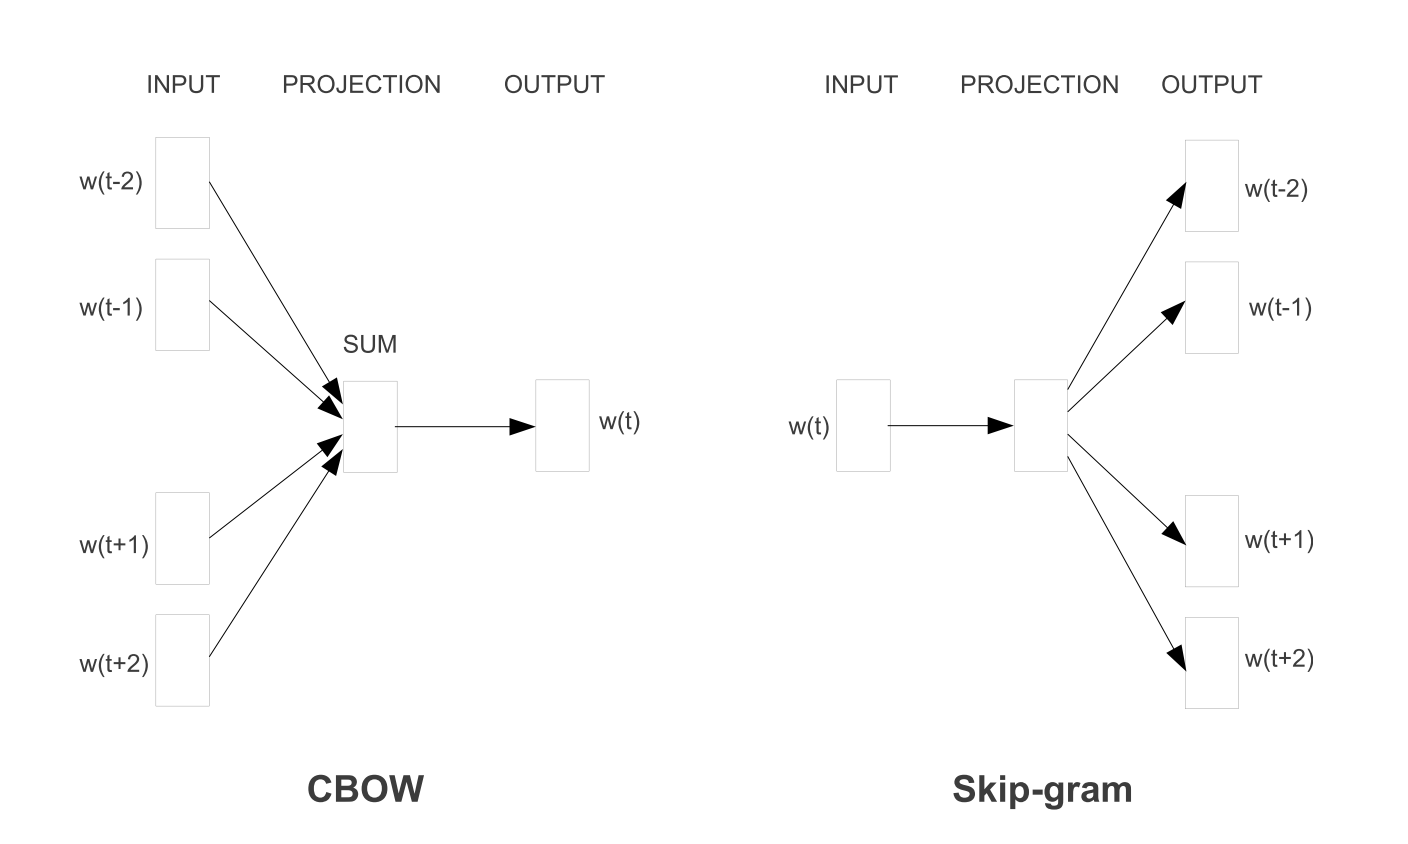
\includegraphics[width=12cm]{kapitel3/cbowskipgr.png}
    \caption[Vergleich zwischen CBOW und Skip-Gram Architektur]{Die CBOW-Architektur sagt das aktuelle Wort basierend auf dem Kontext voraus, während das Skip-Gramm die umgebenden Wörter voraussagt, wenn das aktuelle Wort gegeben ist aus \cite*{Mikolov}).}
    \label{cbowskipgr}
\end{figure}

Der Skip-Gram-Algorithmus ist einer von zwei Algorithmen in einem Softwarepaket namens word2vec, und so wird der Algorithmus manchmal auch als word2vec bezeichnet \cite*{Mikolov2013}\cite*{Mikolov}. Die Intuition von word2vec ist, dass anstatt zu zählen, wie of jedes Wort $w$ in der Nähe von einem anderen Wort vorkommt, einen Klassifikator für eine binäre Vorhersageaufgabe zu trainieren. Die erlernten Klassifikatorgewichte werden dann als Worteinbettungen genommen \cite*[111]{Jurafskya}.

Beim Skip-Gram besteht das Ziel, eine Klassifikation zu trainieren. Dabei wird ein Zielwort $t$ mit Kandidaten aus dem Kontext \textit{c} in ein Tuple gesetzt. \textit{P(+|t,c)} sagt dann aus, wie wahrscheinlich es ist, dass ein Kontextwort \textit{c} ein echter Kontext ist. Zum beispiel sei gegeben der Satz \enquote{Wir essen Spaghetti zum Abendessen...}. Wenn nur der Kontext $\pm 2$ Wörter betrachtet wird, und \textit{t} das Wort \enquote{essen} ist, wird die Klassifikation für das Tuple \textit{(essen,spaghetti)} \enquote{true} und für das Tuple \textit{(essen,auto)} \enquote{false} zurückgeben \cite*[111]{Jurafskya}.

\begin{equation} \label{Formel3_1}
    P(-|t,c) = 1-P(+|t,c)
\end{equation}

Die ähnlichkeit eines Wortes zu einem anderen Wort, kann berechnet werden, indem das Skalarprodukt berechnet wird. Dies ist zunächst nur eine Zahl zwischen $-\infty$ und $+\infty$. Um aus diesem Produkt eine Wahrscheinlichkeit zu berechnen, wird die \textbf{\textit{sigmoid}} Funktion $\sigma(x)$ angewendet. Die Logistikfunktion gibt eine Zahl zwischen0 und 1 zurück. Um die Wahrscheinlichkeit zu berechnen, muss gewährleistet werden, dass die Summe \textit{c ist das Kontextwort} und \textit{c ist nicht das Kontextwort} eine 1 ergeben \cite*[112]{Jurafskya}.

\begin{equation} \label{Formel3_2}
    P(-|t,c) = 1-P(+|t,c) = \frac{e^{-t\cdot c}}{1+e^{-t\cdot c}}
\end{equation}

Skip-Gramm macht die starke, aber sehr nützliche vereinfachende Annahme, dass alle Kontextwörter unabhängig sind, so dass ihre Wahrscheinlichkeiten multipliziert werden können:

\begin{equation} \label{Formel3_3}
    P(+|t,c_{1:k}) = \prod ^{k}_{i=1}\frac{1}{1+e^{-t\cdot c_{i}}}
\end{equation}

\begin{equation} \label{Formel3_4}
    \log P(+|t,c_{1:k}) =\sum ^{k}_{i=1} \log \frac{1}{1+e^{-t\cdot c_{i}}}.
\end{equation}


Skip-Gramm trainiert einen probabilistischen Klassifikator, der einem Zielwort und seinem Kontextfenster eine Wahrscheinlichkeit zuweist, die darauf basiert, wie ähnlich dieses Kontextfenster dem Zielwort ist. Die Wahrscheinlichkeit basiert auf der Anwendung der logistischen Sigmoidfunktion auf das Punktprodukt der Einbettungen des Zielworts mit jedem Kontextwort \cite*[113]{Jurafskya}.

Word2vec lernt Einbettungen, indem es mit einem anfänglichen Satz von Einbettungsvektoren beginnt und dann die Einbettung jedes Wortes $w$ iterativ verschiebt, um mehr den Einbettungen von Wörtern zu ähneln die in der Nähe der Wörter vorkommen. Für das Training eines binären Klassifikators werden negative Beispiele nötig sein. Das Skip-Gram benötigt mehr negative als positive Beispiele für das Training. Das Verhältnis zwischen positiven und negativen Beispielen wird mit einem Parameter $k$ festgelegt. Für jedes der Trainingseinheiten \textit{t, c} werden \textit{k} negative Stichproben erstellt, die jeweils aus dem Ziel \textit{t} plus einem \enquote{noise word} besteht. EIn \enquote{noise word} is ein zufälliges Wort aus dem Lexikon, das nicht das Zielwort \enquote{t} sein darf \cite*[113]{Jurafskya}.

Das Ziel des Lernalgorithmus besteht darin, mittels gegebenen positiven und negativen Beispielen diese Einbettungen so anzupassen, dass die Ähnlichkeit der Ziel- und Kontextwortpaare \textit{(t, c)} aus den positiven Beispielen maximiert werden und die Ähnlichkeit der Paare \textit{(t, c)} aus den negativen Beispielen minimiert wird. Formell lässt sich dieses mit folgender Formel ausdrücken:

\begin{gather} \label{Formel3_5}
    L(\theta) = \sum_{(t,c)\in +}\log P(+|t,c)+\sum_{(t,c)\in -} \log P(-|t,c) =  \notag\\
    \log \sigma(c \cdot t)+\sum^{k}_{i=1}\log \sigma(-n_{i} \cdot t) = \notag\\
    \log \frac{1}{1+e^{-c \cdot t}}+\sum^{k}_{i=1}\log\frac{1}{1+e^{n_{1} \cdot t}}.
\end{gather}

Das heißt, wir möchten das Punktprodukt des Wortes mit den tatsächlichen Kontextwörtern maximieren und die Punktprodukte des Wortes mit den k negativen Nichtnachbarwörtern minimieren. Wir können dann den stochastischen Gradientenabstieg verwenden, um dieses Ziel zu erreichen, indem wir die Parameter (die Einbettungen für jedes Zielwort $t$ und jedes Kontextwort oder \enquote{noise word} $c$ im Vokabular) iterativ modifizieren \cite*[114]{Jurafskya}.

% \subsubsection{Glove}
% Eine andere Methode zum Einbetten von Wörtern ist Glove (\enquote{Global Vectors}). Es basiert auf Matrixfaktorisierungstechniken für die Wortkontextmatrix. Zunächst wird eine große Matrix von Informationen zum gleichzeitigen Auftreten von Wörter und Kontext erstellt, d. H. für jedes \enquote{Wort} (die Zeilen) wird gezählt, wie häufig dieses Wort in einem \enquote{Kontext} (den Spalten) in einem großen Korpus angezeigt wird. Dann wird diese Matrix in eine niederdimensionale Matrix Wort und Merkmale zerlegt, in der jede Zeile nun eine Vektordarstellung für jedes Wort speichert. Dies geschieht im Allgemeinen durch Minimierung eines \enquote{Rekonstruktionsverlusts}. Dieser Verlust versucht, die niederdimensionalen Darstellungen zu finden, die den größten Teil der Varianz in den hochdimensionalen Daten erklären können.




% \chapter{Grobe Zeit- und Ressourcenplanung}
% % \label{Kap3}
% Grobe Zeitplanung und die Anteile der Kapitel and er Arbeit:
% \begin{itemize}
%     \item \textbf{November 2020 bis Oktober 2020:} Kapitel 2, 3 (ca. 25\%)
%     \item \textbf{Dezember 2020} Kapitel 4-5 (ca. 25\%)
%     \item \textbf{Januar 2021:} Kapitel 6 (ca. 20\%)
%     \item \textbf{Februar 2021:} Kapitel 7 (ca. 20\%)
%     \item \textbf{März 2021:} Kapitel 1, 8 (ca. 10\%)
% \end{itemize}
% \section{Bilder}

% Natürlich können auch Grafiken und Bilder eingebunden werden, siehe z.\,B. Abbildung~\ref{Kap2:NasaRover}.

% \begin{figure}[ht]
%     \centering
%     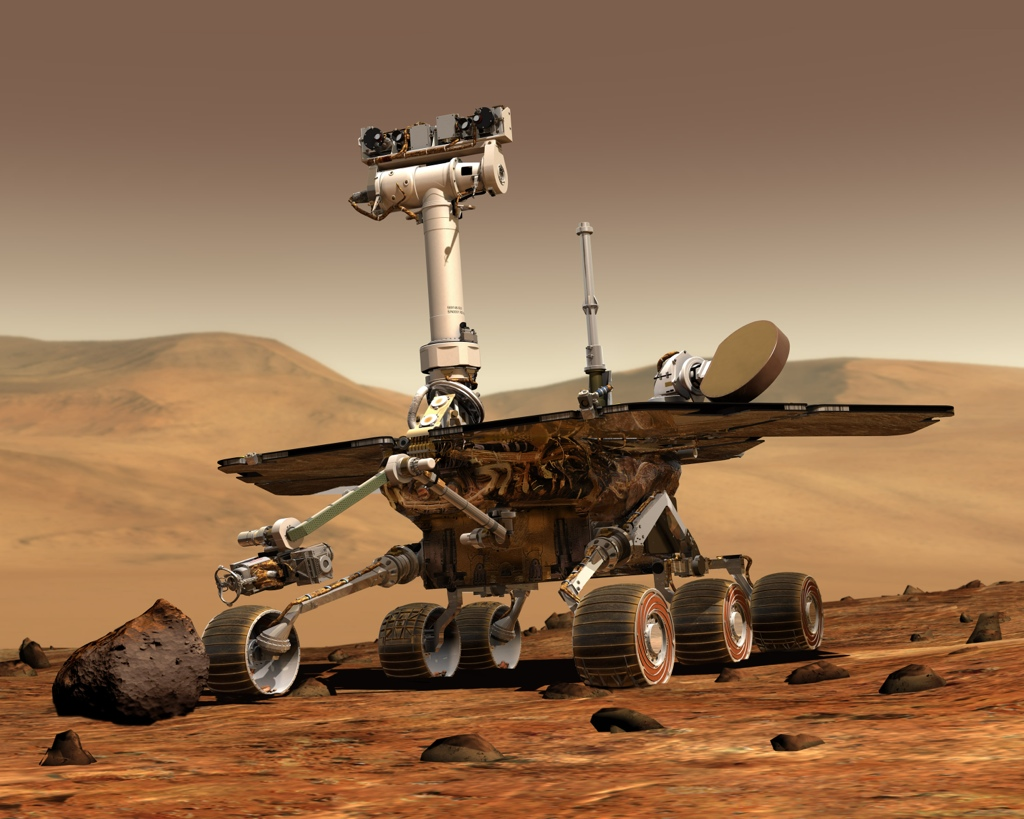
\includegraphics[width=6cm]{kapitel3/nasa_rover}
%     \caption{Ein Nasa Rover}
%     \label{Kap2:NasaRover}
% \end{figure}

% Man kann sich auch selbst ein Makro für das Einfügen von Bildern schreiben:

% \bild{kapitel3/modell_point_to_point}{6cm}{Point to Point}

% \begin{sidewaysfigure}
%     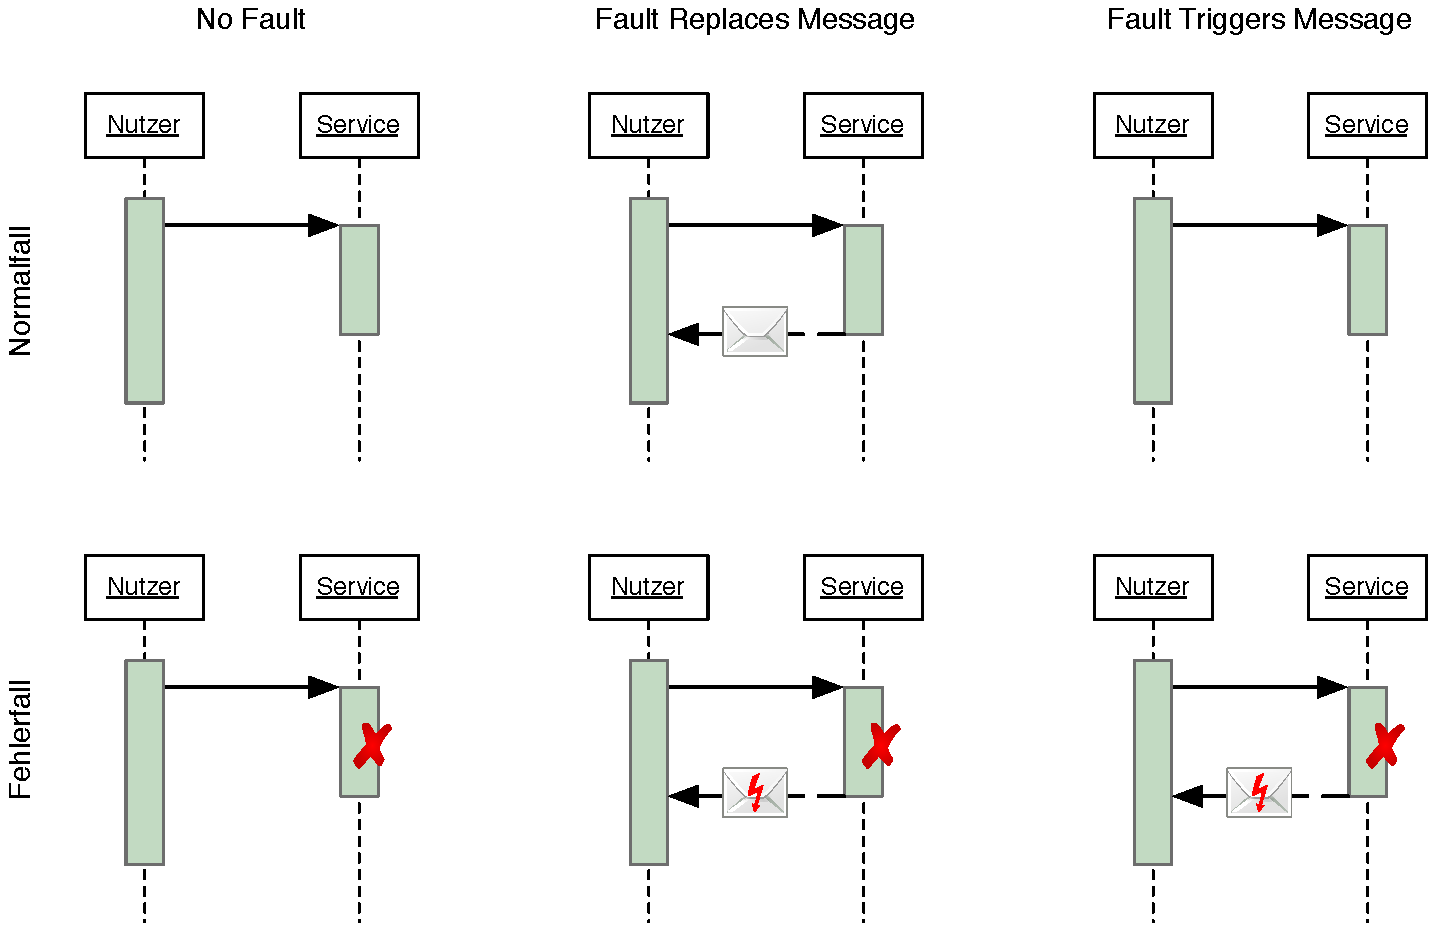
\includegraphics[width=22cm]{kapitel3/ws-wsdl20-fehler}
%     \caption{Sehr große Grafiken kann man drehen, damit sie auf die Seite passen}
%     \label{Kap2:wsdl-fehler}
% \end{sidewaysfigure}

% \clearpage % Alle Bilder, die bisher kamen ausgeben


% \section{Formelsatz}

% Eine Formel gefällig? Mitten im Text $a_2 = \sqrt{x^3}$ oder als eigener Absatz (siehe Formel~\ref{Formel}):

% \begin{equation}
%     \begin{bmatrix}
%         1 & 4 & 2  \\
%         4 & 0 & -3
%     \end{bmatrix}
%     \cdot
%     \begin{bmatrix}
%         1  & 1 & 0 \\
%         -2 & 3 & 5 \\
%         0  & 1 & 4
%     \end{bmatrix}
%     {=}
%     \begin{bmatrix}
%         -7 & 15 & 28  \\
%         4  & 1  & -12
%     \end{bmatrix}
%     \label{Formel}
% \end{equation}


% \section{Sourcecode}

% Man kann mit Latex auch ganz toll Sourcecode in den Text aufnehmen.

% \subsection{Aus einer Datei}

% \lstinputlisting[firstline=2,language=Java,caption={Crypter-Interface},label=lst:CrypterInterface]{\srcloc/Crypter.java}


% \subsection{Inline}

% \begin{lstlisting}[language=Java,caption=Methode checkKey()]
%     /**
%      * Testet den Schlüssel auf Korrektheit: Er muss mindestens die Länge 1
%      * haben und darf nur Zeichen von A-Z enthalten.
%      *
%      * @param key zu testender Schlüssel
%      * @throws CrypterException wenn der Schlüssel nicht OK ist.
%      */
%     protected void checkKey(Key key) throws CrypterException {

%         // Passt die Länge?
%         if (key.getKey().length == 0) {
%             throw new CrypterException("Der Schlüssel muss mindestens " +
%                     "ein Zeichen lang sein");
%         }

%         checkCharacters(key.getKey(), ALPHABET);
%     }
% \end{lstlisting}


% \section{Anforderungen}

% Anforderungen im Format des Volere"=Templates (Snowcards) \autocite{Volere} können per Makro eingefügt werden. Das Label wird automatisch mit der Nummer erstellt, d.\,h. Sie können auf die Tabelle mit dieser referenzieren (siehe \autoref{F52}).

% \snowcard % Snowcard einbinden (Anpassungen in titelblatt.tex)
% {F52} % Nummer des Requirements
% {F} % Art
% {Hoch} % Priorität
% {User Authentifizierung} % Titel
% {Interview mit Abteilungsleiter} % Herkunft (Optional)
% {F12} % Konflikte (Optional)
% {Der Benutzer ist in der Lage sich über seinen
%     Benutzernamen und sein Passwort am System anzumelden} % Beschreibung
% {Ein Benutzer kann sich mit seinem firmenweiten Benutzernamen und
%     Passwort über die Anmeldemaske anmelden und hat Zugriff auf die
%     Funktionen des Systems} % Fit-Kriterium (Optional)
% {Benutzerhandbuch des Altsystems} % Material (Optional)

% Ebenso können Sie nicht"=funktionale Anforderungen mit Hilfe von Quality Attribute Scenarios (vgl. \autoref{NF11}) darstellen. Zu Details siehe \autocite{Barbacci2003}.

% \qas % Quality-Attribute Scenario einbinden (Anpassungen in titelblatt.tex)
% {NF11} % Nummer des Requirements
% {Hoch} % Priotität
% {Performance des Jahresabschlusses} % Titel
% {Endbenutzer} % Quelle
% {Startet einen Jahresabschluss} % Stimulus
% {Buchhaltungssystem} % Artefakt
% {Das System befindet sich im normalen Betriebszustand} % Umgebung
% {Jahresabschluss ist durchgeführt und kann als PDF abgerufen werden} % Antwort
% {10 Minuten} % Antwort-Maß

% Die Abgrenzung von funktionalen und nicht-funktionalen Anforderungen ist nicht immer einfach und bereitet manchen Studierenden Probleme. Als Hilfestellung kann die von der ISO25010 \autocite{ISO25010} zur Verfügung gestellte Liste dienen, siehe \autoref{kapitel3/iso25010}.

% \bild{kapitel3/iso25010}{14cm}{Qualitätsmodell für Software-Produkte nach ISO25010}

% \citeauthor{Bass2003} listen in \autocite{Bass2003} eine ähnliche Liste von Kategorien für nicht-funktionalen Anforderungen auf, die ebenfalls als Richtschnur dienen kann. Diese sind:

% \begin{itemize}
%     \item \textit{Verfügbarkeit} \textit{(availability)} -- umfasst Zuverlässigkeit (reliability), Robustheit (robustness), Fehlertoleranz (fault tolerance) und Skalierbarkeit (scalability)
%     \item \textit{Anpassbarkeit} \textit{(modifiability)}, umfasst Wartbarkeit (maintainability), Verständlichkeit (understandability) und Portabilität (portability).
%     \item \textit{Performanz} \textit{(performance)}
%     \item \textit{Sicherheit} \textit{(security)}
%     \item \textit{Testbarkeit} \textit{(testability)}
%     \item \textit{Bedienbarkeit} \textit{(usability)}
% \end{itemize}
